%\section{More Simulation Results}\label{appendix:more_result}
\section{More Numerics}\label{appendix:more_result}

This section provides more numerical results on simulated datasets
in \ref{fig:vary-k-400-app},
\ref{fig:vary-k-200-app},
\ref{fig:vary-k-400-compare-app},
and \ref{fig:vary-k-200-compare-app}.

\begin{figure}
	\centering
	\begin{subfigure}{0.3\textwidth}
		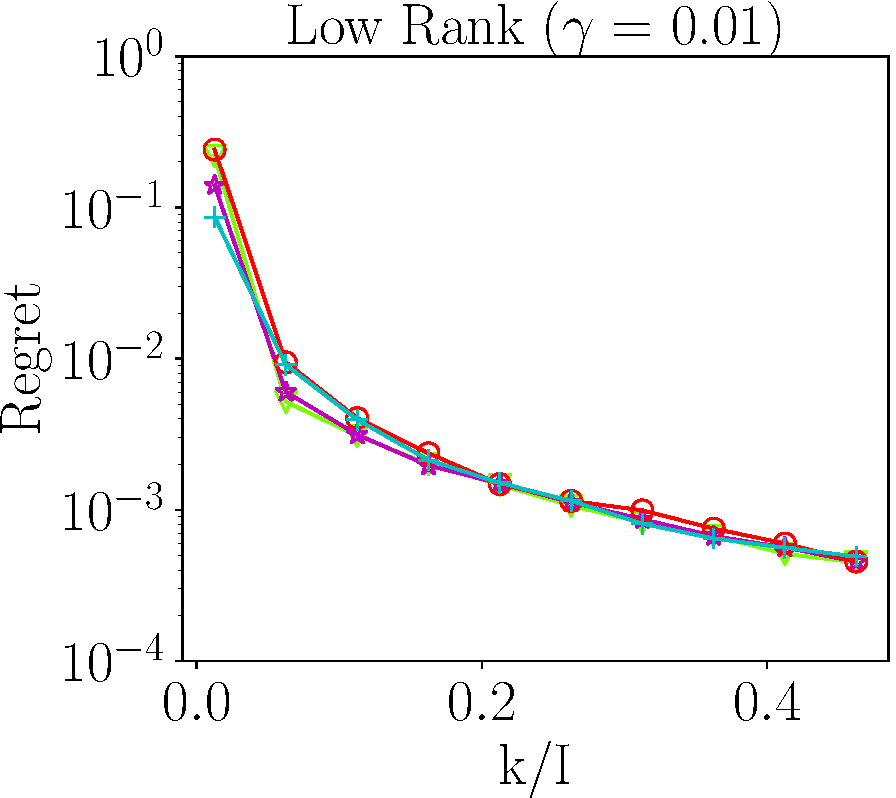
\includegraphics[scale = 0.24]{figure/fig2_lk_lnoise_400.pdf}
	\end{subfigure}
	\begin{subfigure}{0.3\textwidth}
		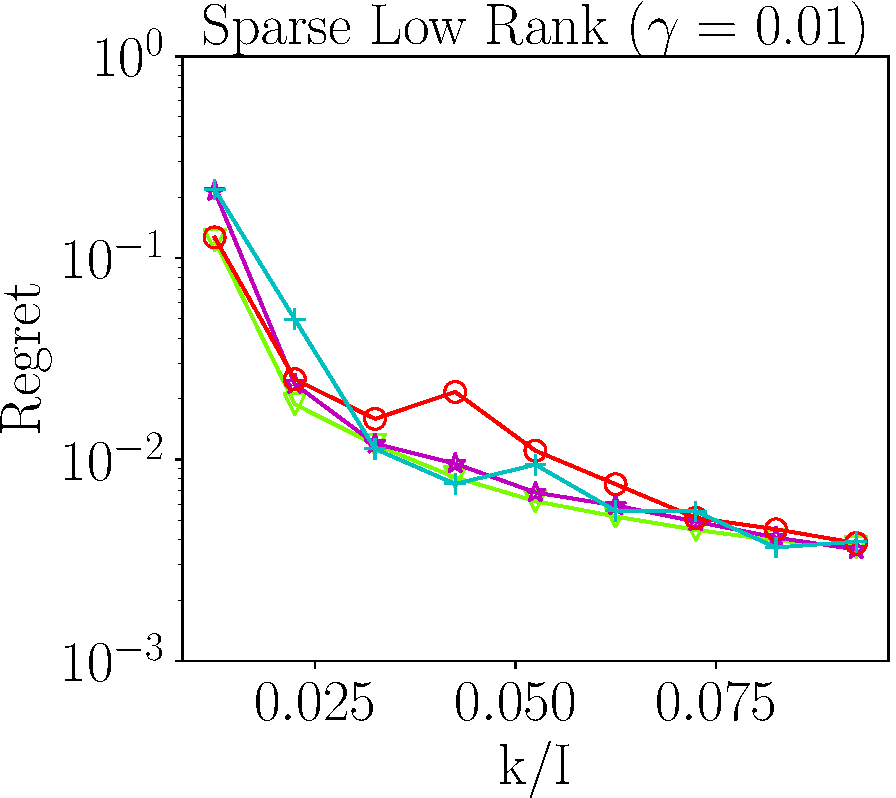
\includegraphics[scale = 0.24]{figure/fig2_slk_lnoise_400.pdf}
	\end{subfigure}
	\begin{subfigure}{0.3\textwidth}
		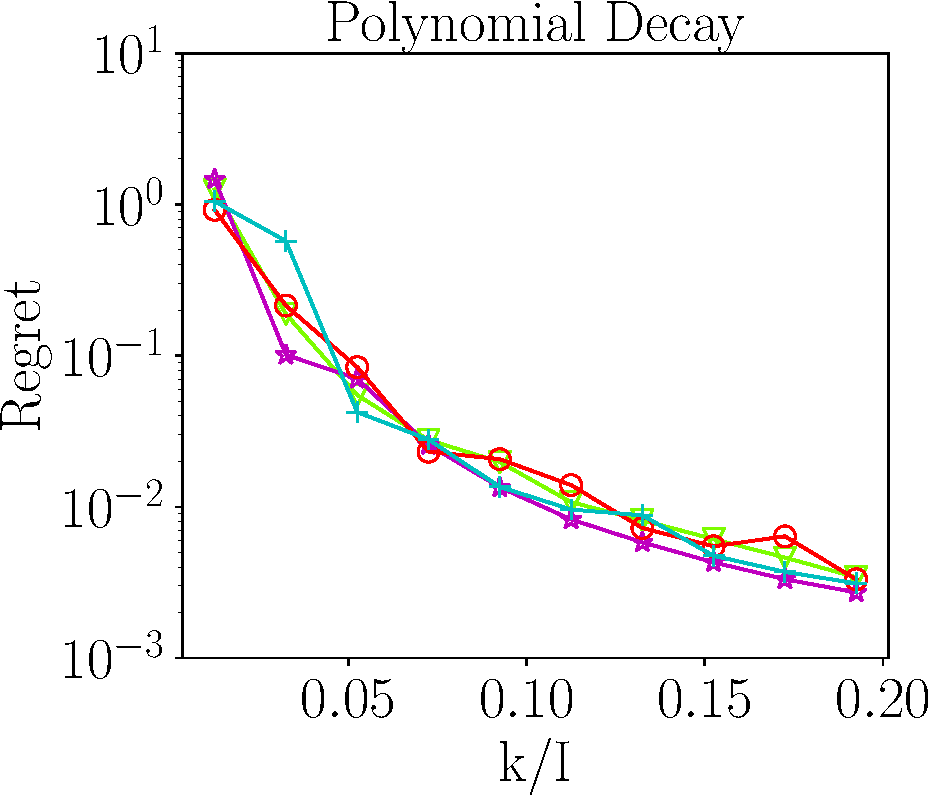
\includegraphics[scale = 0.24]{figure/fig2_spd_400.pdf}
	\end{subfigure}\\
	\begin{subfigure}{0.3\textwidth}
		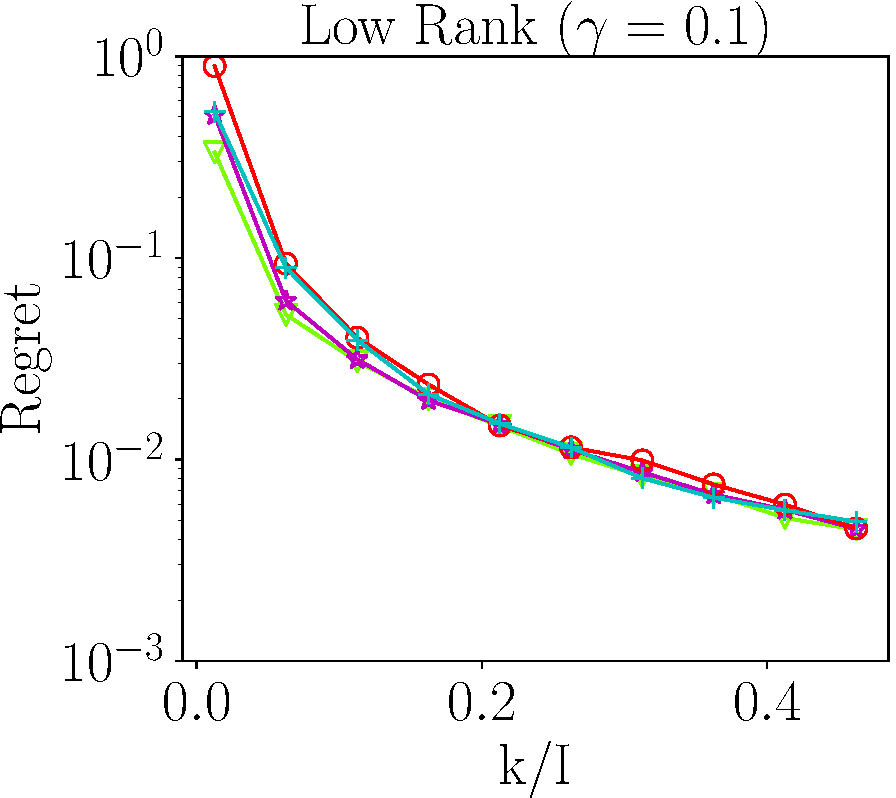
\includegraphics[scale = 0.24]{figure/fig2_lk_mnoise_400.pdf}
	\end{subfigure}
	\begin{subfigure}{0.5\textwidth}
		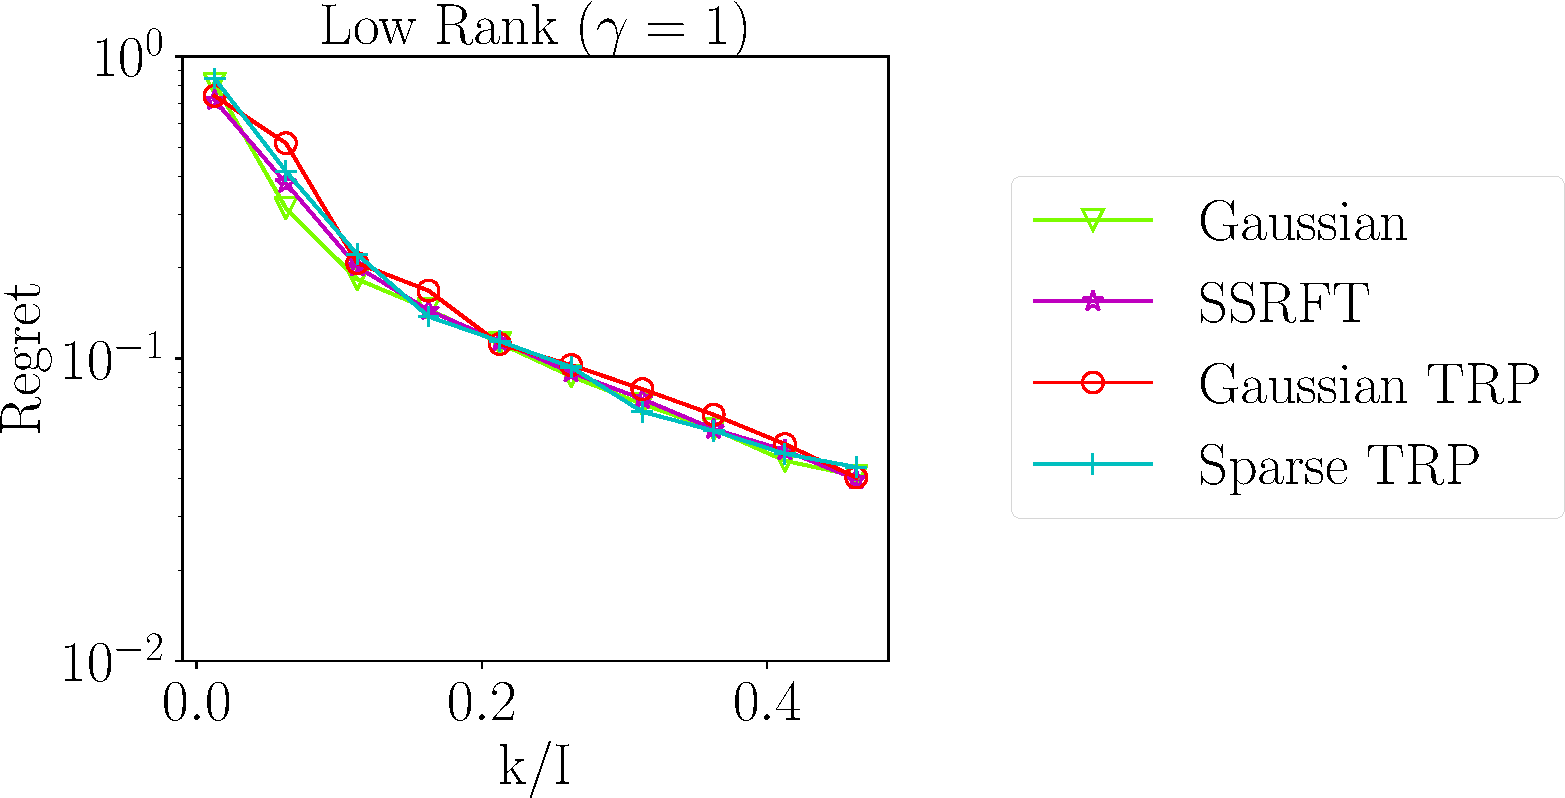
\includegraphics[scale = 0.24]{figure/fig2_lk_hnoise_400.pdf}
	\end{subfigure}
	\caption{We approximate 3D synthetic tensors (see \ref{s-synthetic-data}) with $I = 400$,
		using our one-pass algorithm with $r = 5$ and varying $k$ ($s = 2k+1$),
		using a variety of DRMs in the Tucker sketch:
		Gaussian, SSRFT, Gaussian TRP, or Sparse TRP.}
		\label{fig:vary-k-400-app}
\end{figure}



\begin{figure}
	\centering
	\begin{subfigure}{0.3\textwidth}
		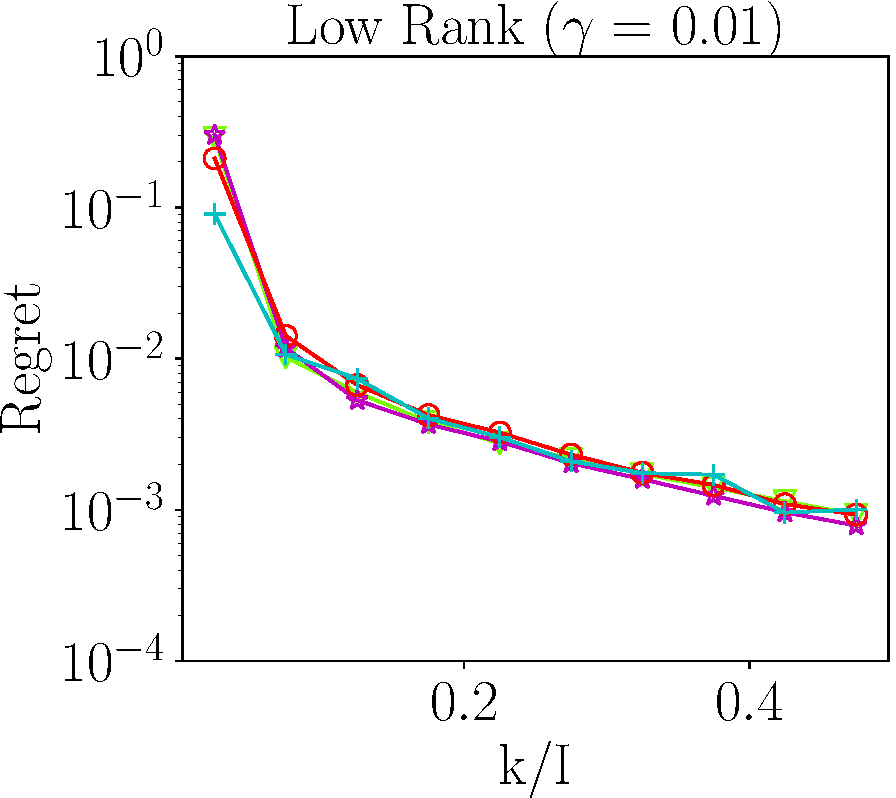
\includegraphics[scale = 0.25]{figure/fig2_lk_lnoise_200.pdf}
	\end{subfigure}
	\begin{subfigure}{0.3\textwidth}
		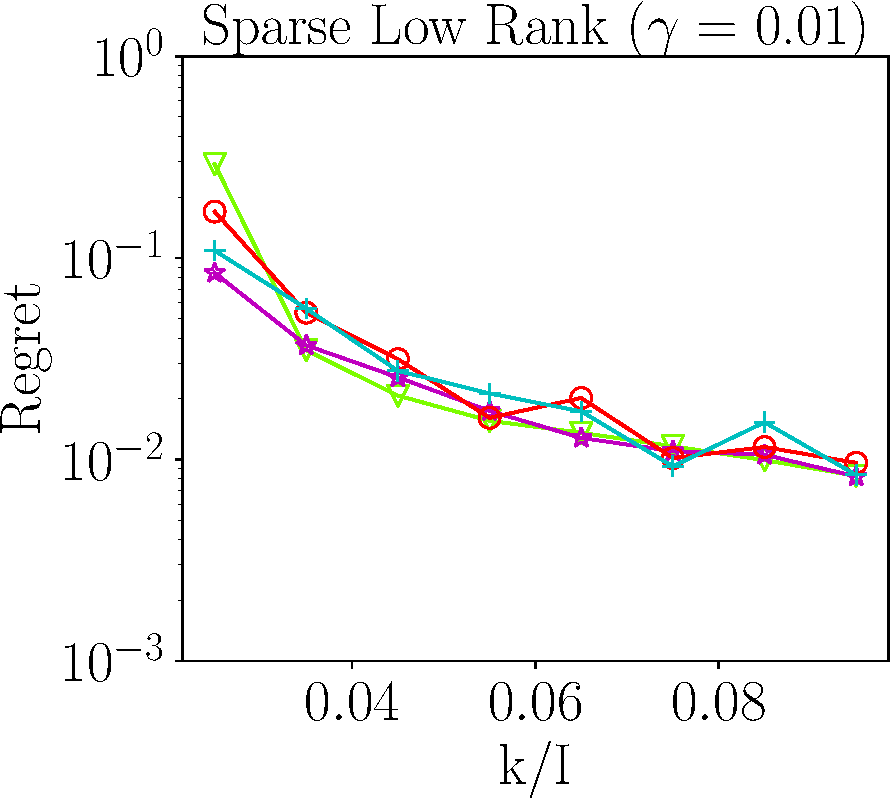
\includegraphics[scale = 0.25]{figure/fig2_slk_lnoise_200.pdf}
	\end{subfigure}
	\begin{subfigure}{0.3\textwidth}
		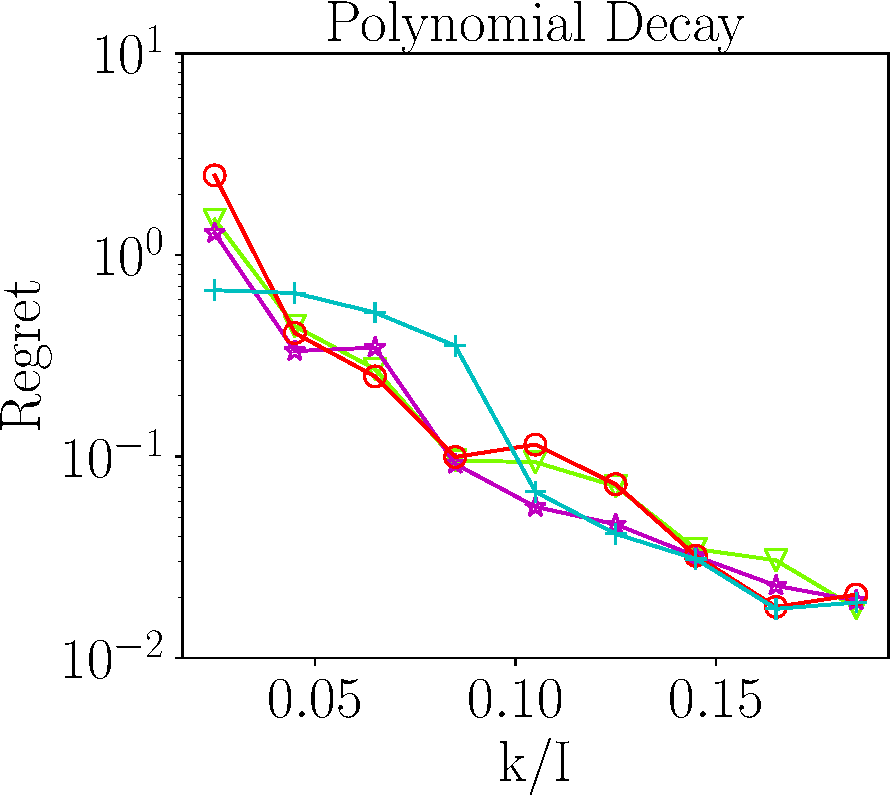
\includegraphics[scale = 0.25]{figure/fig2_spd_200.pdf}
	\end{subfigure}\\
	\begin{subfigure}{0.3\textwidth}
	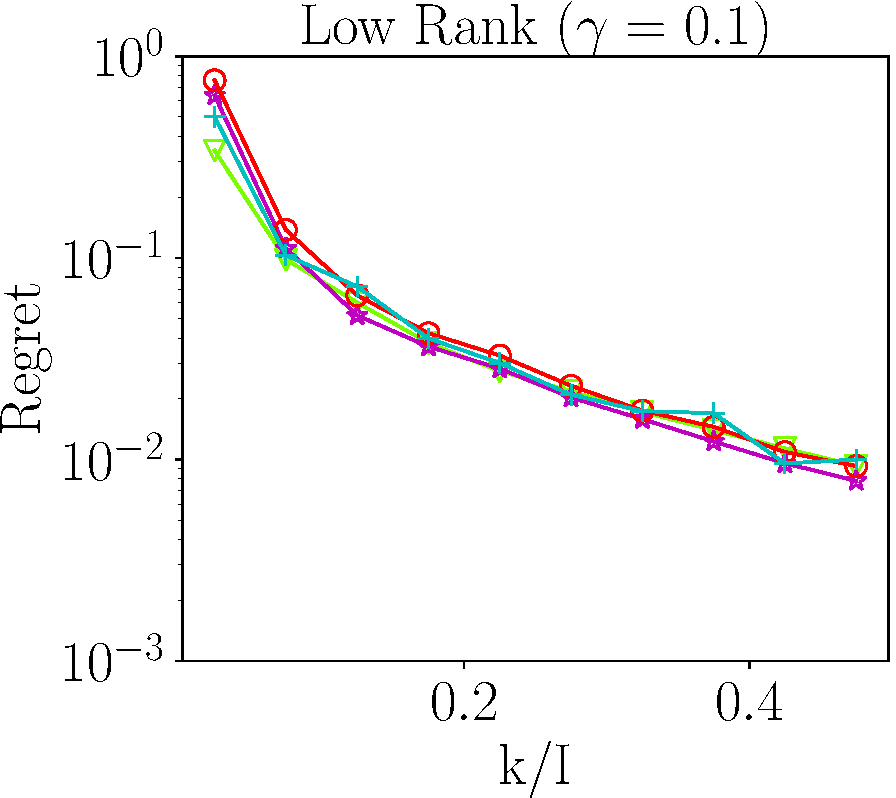
\includegraphics[scale = 0.25]{figure/fig2_lk_mnoise_200.pdf}
	\end{subfigure}
	\begin{subfigure}{0.55\textwidth}
		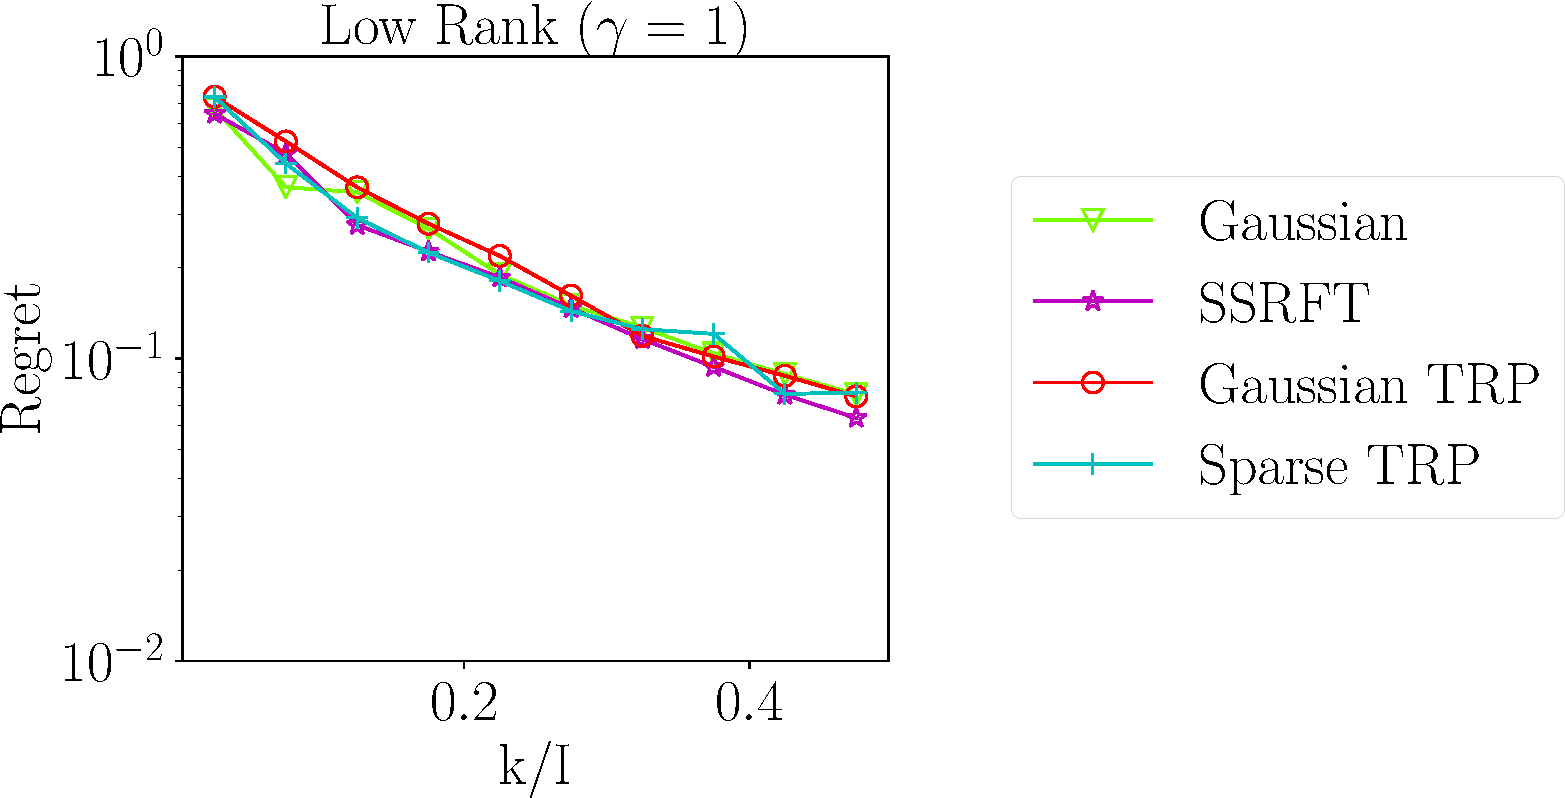
\includegraphics[scale = 0.25]{figure/fig2_lk_hnoise_200.pdf}
	\end{subfigure}
	\caption{We approximate 3D synthetic tensors (see \ref{s-synthetic-data}) with $I = 200$,
		using our one-pass algorithm with $r = 5$ and varying $k$ ($s = 2k+1$),
		using a variety of DRMs in the Tucker sketch:
		Gaussian, SSRFT, Gaussian TRP, or Sparse TRP.}
		\label{fig:vary-k-200-app}
\end{figure}

% More comparison for two-pass and one-pass algorithm


\begin{figure}
	\centering
	\begin{subfigure}{0.3\textwidth}
		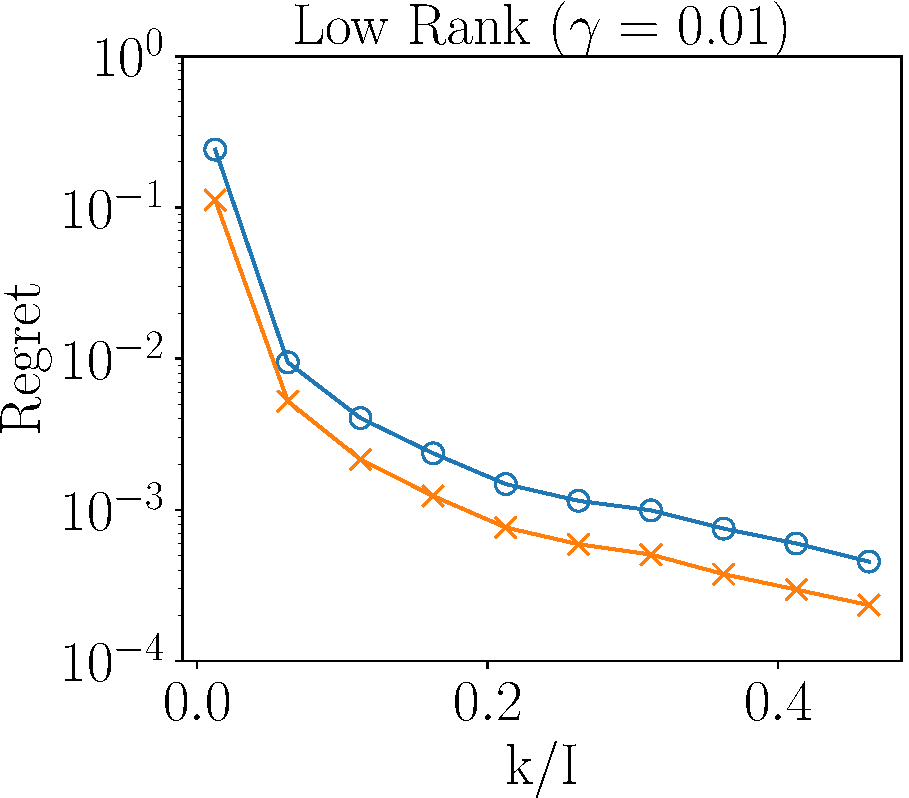
\includegraphics[scale = 0.24]{figure/fig3_lk_lnoise_400.pdf}
	\end{subfigure}
	\begin{subfigure}{0.3\textwidth}
		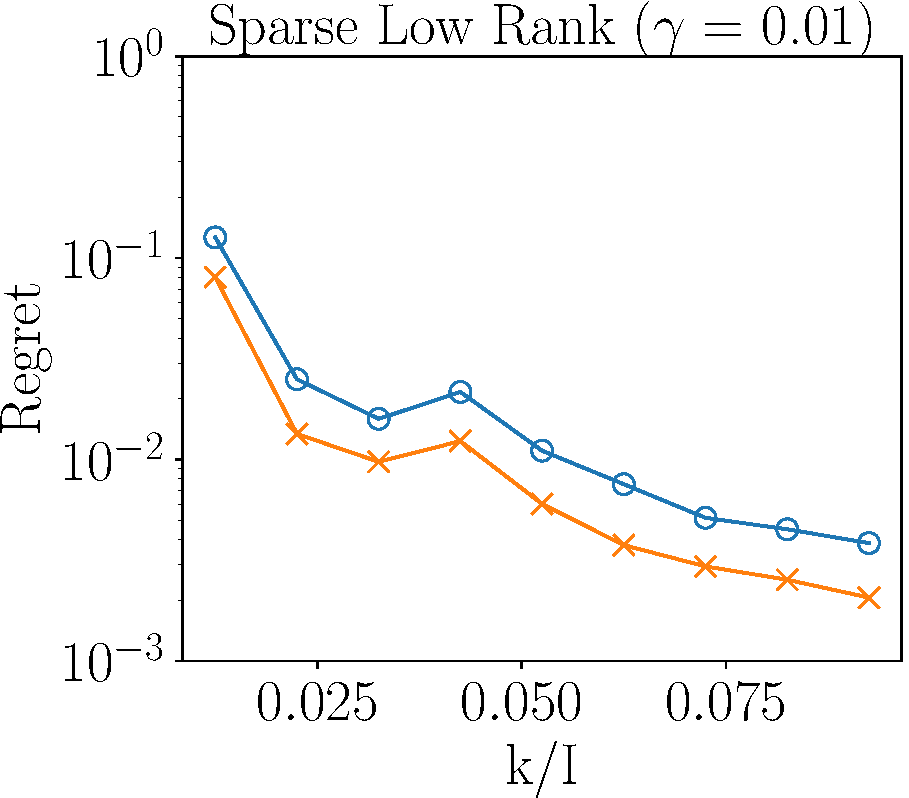
\includegraphics[scale = 0.24]{figure/fig3_slk_lnoise_400.pdf}
	\end{subfigure}
	\begin{subfigure}{0.3\textwidth}
		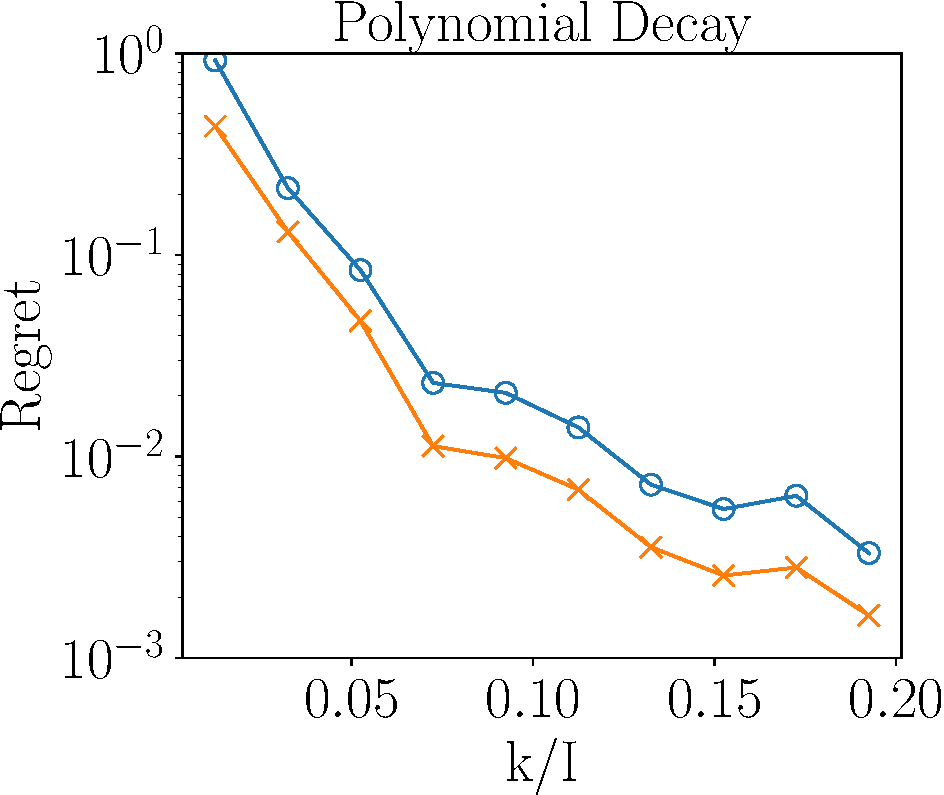
\includegraphics[scale = 0.24]{figure/fig3_spd_400.pdf}
	\end{subfigure}\\
	\begin{subfigure}{0.3\textwidth}
		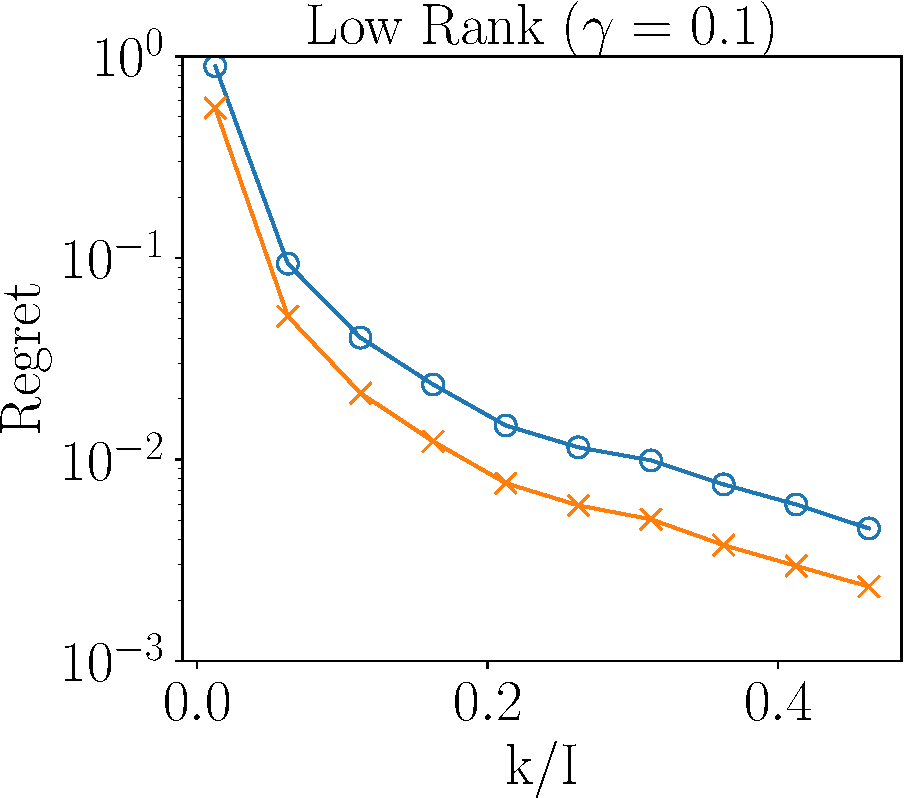
\includegraphics[scale = 0.24]{figure/fig3_lk_mnoise_400.pdf}
	\end{subfigure}
	\begin{subfigure}{0.55\textwidth}
		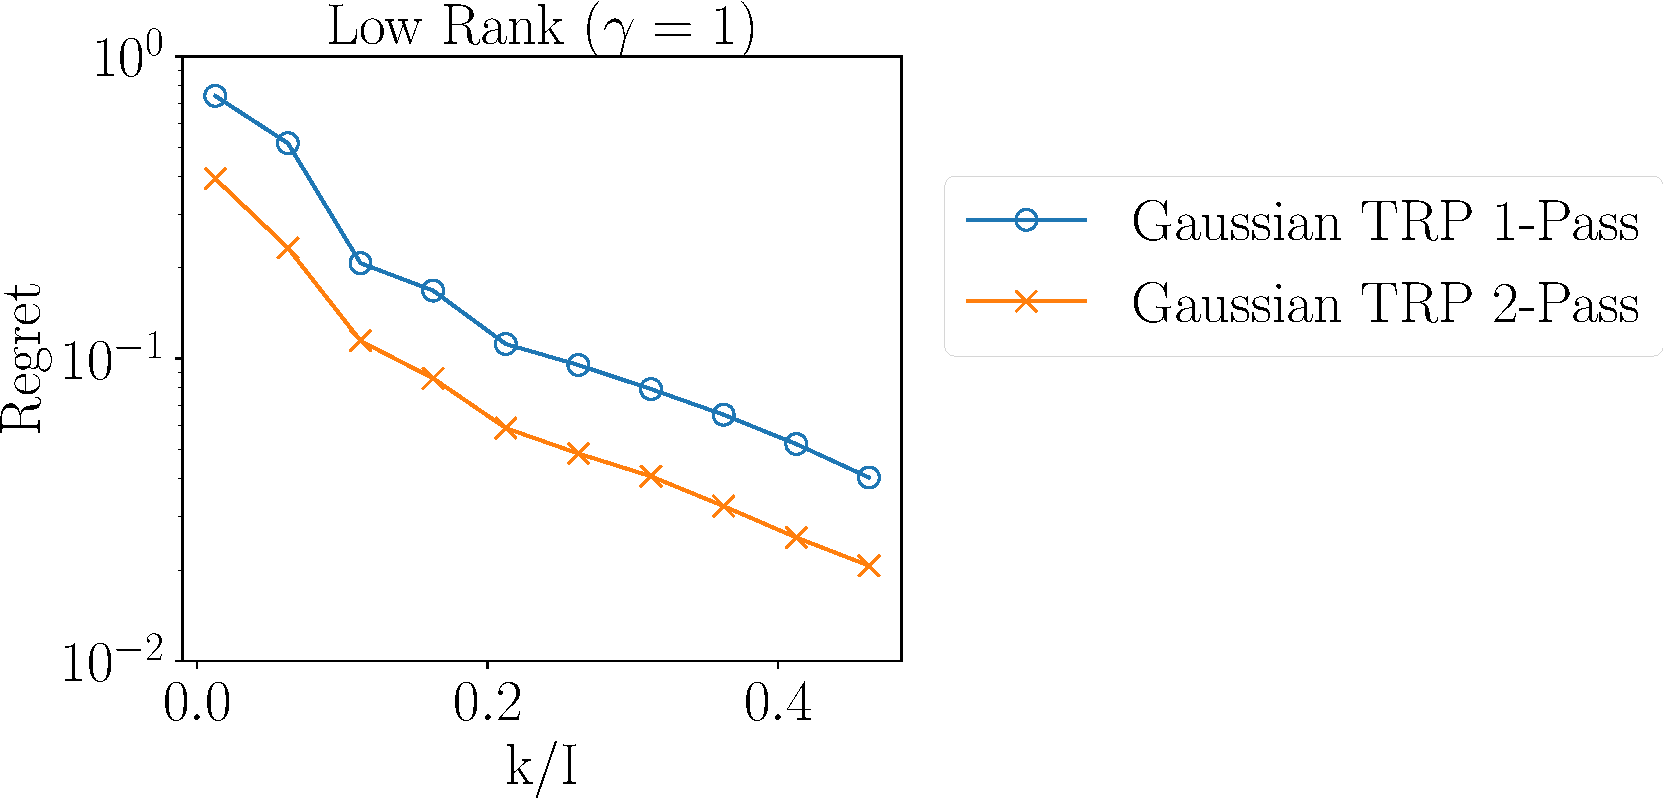
\includegraphics[scale = 0.24]{figure/fig3_lk_hnoise_400.pdf}
	\end{subfigure}
	\caption{We approximate 3D synthetic tensors (see \ref{s-synthetic-data}) with $I = 400$,
		using our one-pass and two-pass algorithms with $r = 5$ and varying $k$ ($s = 2k+1$),
		using the Gaussian TRP in the Tucker sketch.}\label{fig:vary-k-400-compare-app}
\end{figure}



\begin{figure}
	\centering
	\begin{subfigure}{0.3\textwidth}
		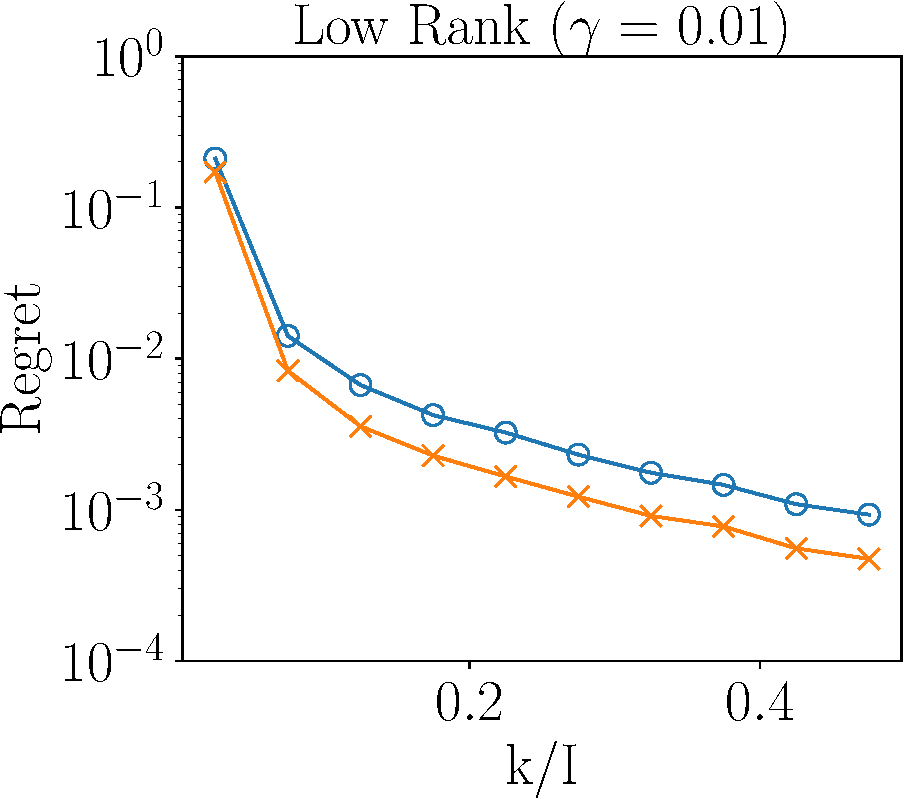
\includegraphics[scale = 0.25]{figure/fig3_lk_lnoise_200.pdf}
	\end{subfigure}
	\begin{subfigure}{0.3\textwidth}
		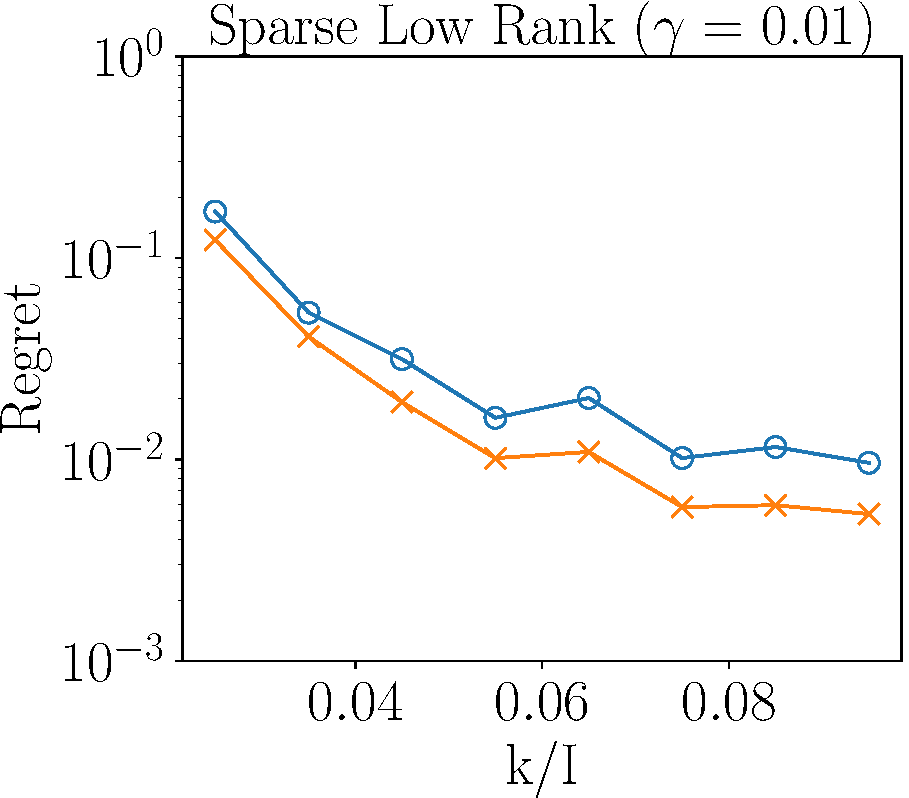
\includegraphics[scale = 0.25]{figure/fig3_slk_lnoise_200.pdf}
	\end{subfigure}
	\begin{subfigure}{0.3\textwidth}
		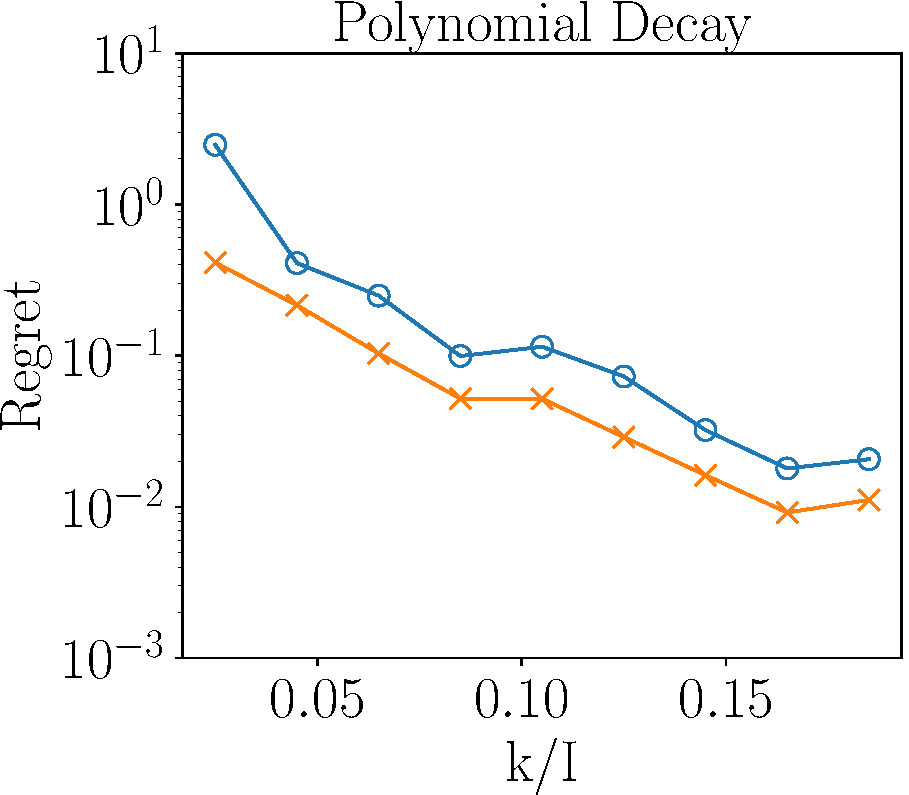
\includegraphics[scale = 0.25]{figure/fig3_spd_200.pdf}
	\end{subfigure}\\
	\begin{subfigure}{0.3\textwidth}
		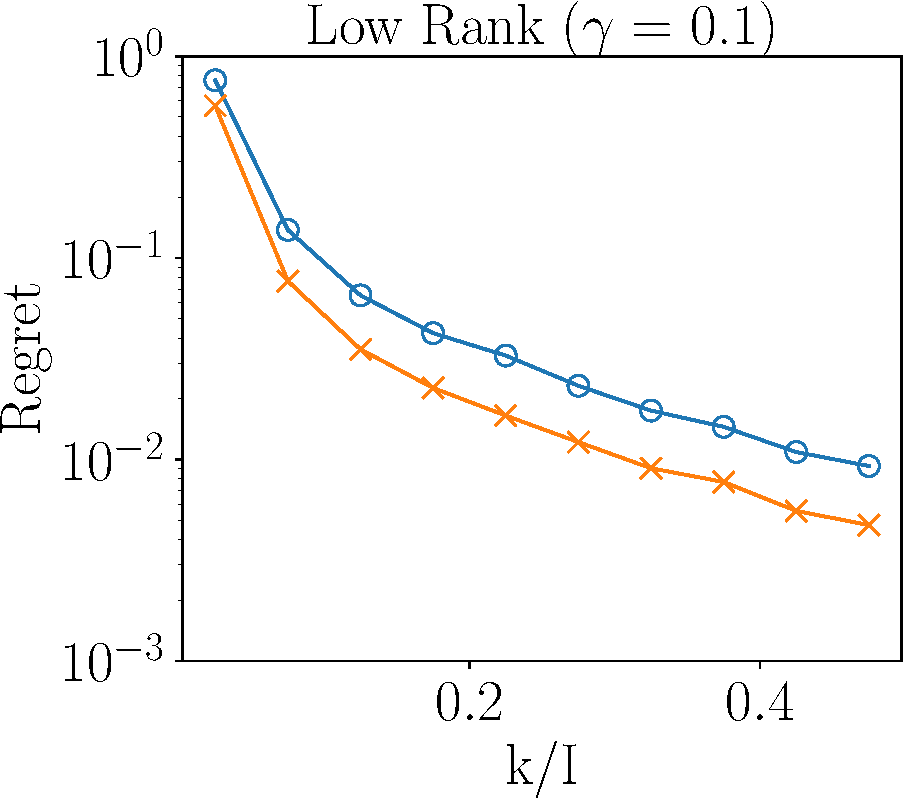
\includegraphics[scale = 0.25]{figure/fig3_lk_mnoise_200.pdf}
	\end{subfigure}
	\begin{subfigure}{0.55\textwidth}
		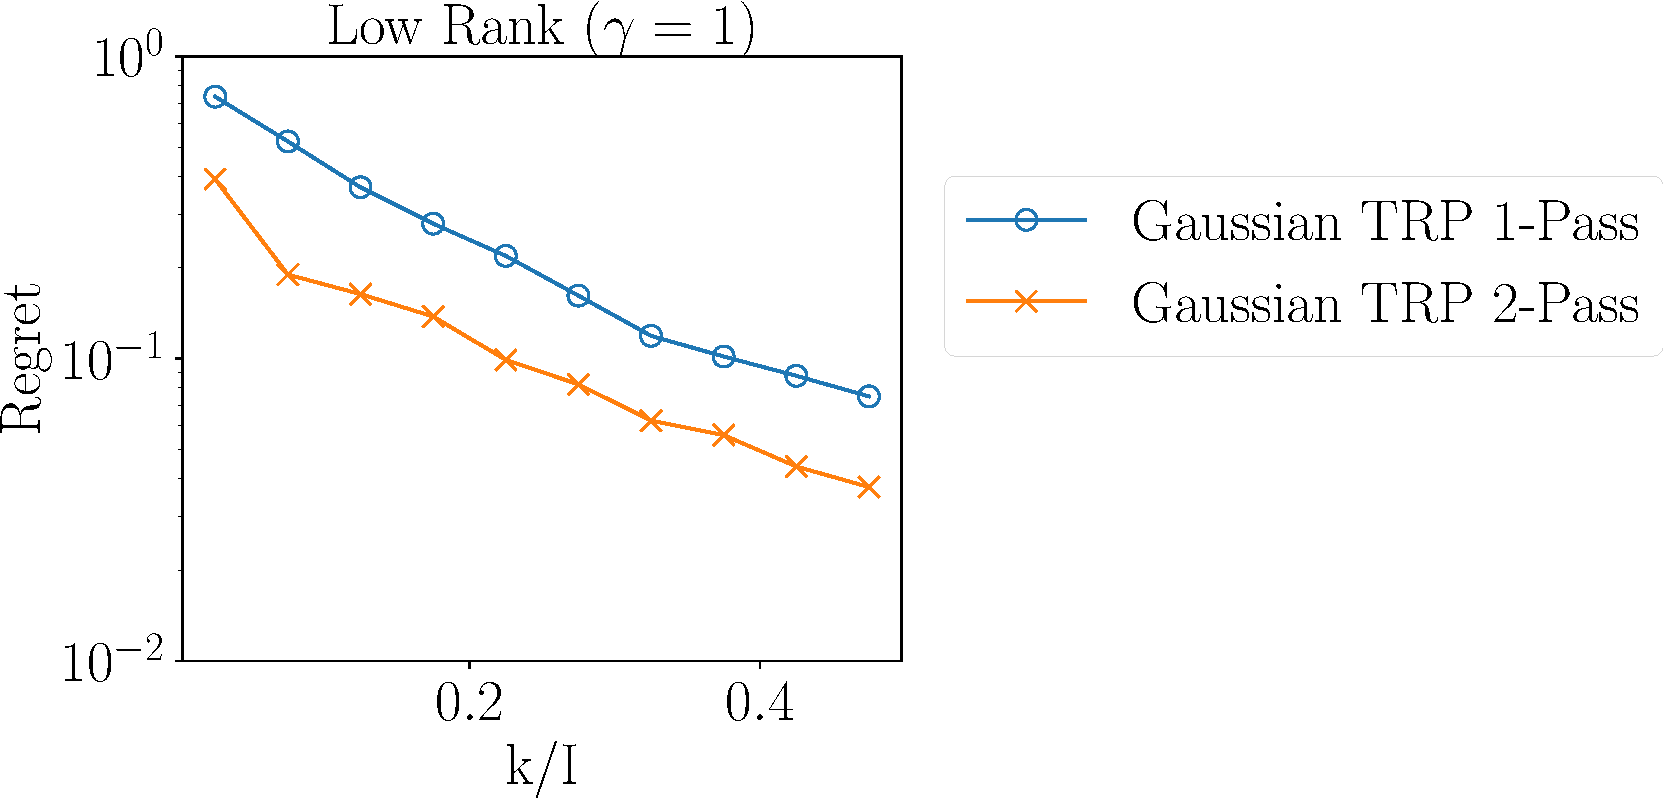
\includegraphics[scale = 0.25]{figure/fig3_lk_hnoise_200.pdf}
	\end{subfigure}
	\caption{We approximate 3D synthetic tensors (see \ref{s-synthetic-data}) with $I = 200$,
		using our one-pass and two-pass algorithms with $r = 5$ and varying $k$ ($s = 2k+1$),
		using the Gaussian TRP in the Tucker sketch.}\label{fig:vary-k-200-compare-app}

\end{figure}
